\subsection{The Heat Equation}
Fourier Analysis was first discovered when Joseph Fourier first developed the Heat Equation. 
The Heat Equation models the flow of heat along a certain heat profile over time. 
The Heat Equation is more generally known as the Diffusion Equation and is used to model the diffusion of varying concentrations of a substance in space and time.
Thus, this equation has applications in physics, chemistry, biology, engineering, and beyond.
In this example, a 1D solution will be derived and solved \citep{Sanderson_2019}.

\subsubsection{Definition}
\noindent
Let us define a rod with the following assumptions:
\begin{itemize}
    \item The rod is of length \(L\) and is composed of a homogeneous material with a heat diffusion coefficient \( \alpha^2 \).
    \item The rod is perfectly insulated along the Y and Z axes. Thus, heat can only flow along the X-axis of the rod.
    \item The rod is thin enough such that the temperature of the rod at any cross-section is uniform.
    \item The rod is initially at a uniform temperature \(u(x,0) = f(x)\). Thus, the rod temperature at position \(x\) at time \(t\) is \(u(x,t)\).
\end{itemize}

\noindent
Thus, the heat equation in one dimension is defined as follows \citep{Crawford_2022a}:
\begin{equation} \label{eq:heat_equation}
    \frac{\partial u}{\partial t} = \alpha^2 \nabla^2 u = \alpha^2 \frac{\partial^2 u}{\partial x^2}
\end{equation}

\noindent
Or in subscript notation,
\begin{equation} \label{eq:heat_equation_subscript}
    u_t = \alpha^2 u_{xx}
\end{equation}

\subsubsection{Application of the Fourier Transform}
Since \(u(x,t)\) is defined as the temperature of the rod at position \(x\) and time \(t\), we can apply the Fourier Transform to \(u(x,t)\) with respect to position \(x\) to reduce the \cref{eq:heat_equation_subscript} PDE into an ODE. Thus, let \(U(\kappa,t)\) be the Fourier Transform of \(u(x,t)\) with respect to \(x\).

\vspace{5mm}
\noindent
Taking the Fourier Transform of \cref{eq:heat_equation_subscript} with respect to \(x\),
\begin{equation}
    \mathcal{F}_x \left\{ u_t \right\} = \mathcal{F}_x \left\{ \alpha^2 u_{xx} \right\}
\end{equation}

\noindent
Using \cref{fourier_scaling},
\begin{equation}
    \mathcal{F}_x \left\{ u_t \right\} = \alpha^2 \mathcal{F}_x \left\{ u_{xx} \right\}
\end{equation}

\noindent
Using \cref{fourier_derivative},
\begin{align}
    \mathcal{F}_x \left\{ \frac{\partial^2 u(x, t)}{\partial x^2} \right\} & = i \kappa \mathcal{F}_x \left\{ \frac{\partial u(x, t)}{\partial x} \right\} \\
    & = -\kappa^2 \mathcal{F}_x\{ u(x, t) \} \\
    & = -\kappa^2 U
\end{align}

\noindent
Therefore,
\begin{align}
    \mathcal{F}_x \left\{ u_t \right\} &= -\alpha^2 \kappa^2 U \\
    \frac{dU}{dt} &= -\alpha^2 \kappa^2 U \label{eq:heat_equation_fourier}
\end{align}

\subsubsection{Initial and Boundary Conditions}
\noindent
A simple square waveform will be used as the initial rod temperature for the ODE:
\begin{align}
    u(x, 0) = \label{eq:heat_equation_initial_condition}
    \begin{cases}
        0 & \text{if } 0 \leq x < \frac{2L}{5} \\
        1 & \text{if } \frac{2L}{5} \leq x \leq \frac{3L}{5} \\
        0 & \text{if } \frac{3L}{5} < x \leq L
    \end{cases}
\end{align}

\noindent
Since no heat can diffuse out of the ends of the rod, the following boundary conditions must be true.
\begin{align}
    u_x(0, t) = u_x(L, t) = 0
\end{align}

\subsubsection{Numerical Solution to Heat Equation}
\cref{eq:heat_equation_fourier} is a first-order ODE that can be easily numerically integrated. A numerical solution to \cref{eq:heat_equation_fourier} using a fifth-order Runge-Kutta approximation in Python is presented below. The Python code can be found in \cref{code:heat_equation}.

\begin{figure}[H]
    \centering
    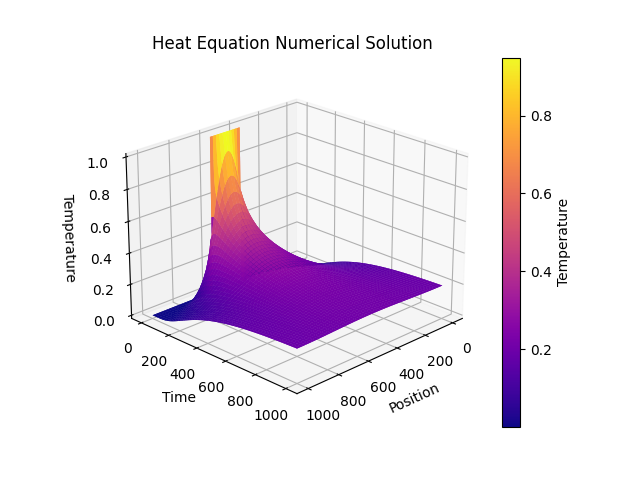
\includegraphics[width=100mm,height=\textheight,keepaspectratio]{images/heat_equation_numerical.png}
    \caption{Using \cref{eq:heat_equation_initial_condition} as the initial temperature function of the rod, this plot shows the temperature change along \(x\) and \(t\) by performing a numerical integration of \cref{eq:heat_equation_fourier}.}
    \label{fig:heat_equation_numerical}
\end{figure}